\documentclass{article}

\usepackage{graphicx}
\usepackage{amsmath}
\usepackage{fancyhdr}
\usepackage{listings}
\usepackage{xcolor}
\usepackage{textcomp}
\usepackage{float}
\usepackage[sorting=none]{biblatex}
\usepackage[margin=1in]{geometry}
\usepackage[font={small,it}]{caption}
\usepackage{placeins}
\usepackage{xepersian}

%\DeclareMathOperator*{\btie}{\bowtie}
\addbibresource{bibliography.bib}
\settextfont[Scale=1.2]{B-NAZANIN.TTF}
\setlatintextfont[Scale=1]{Times New Roman}
\renewcommand{\baselinestretch}{1.5}
\pagestyle{fancy}
\fancyhf{}
\rhead{تکلیف هفتم درس پایگاه داده‌ها 1}
\lhead{\thepage}
\rfoot{علیرضا ابره فروش}
\lfoot{9816603}
\renewcommand{\headrulewidth}{1pt}
\renewcommand{\footrulewidth}{1pt}
%%%%%%%%%%
\lstset
{
    language=[latex]tex,
    basicstyle=\ttfamily,
    commentstyle=\color{black},
    columns=fullflexible,
    keepspaces=true,
    upquote=true,
    showstringspaces=false,
    morestring=[s]\\\%,
    stringstyle=\color{black},
}
%%%%%%%%%%

\begin{document}
\begin{titlepage}
\begin{center}

\includegraphics[width=0.4\textwidth]{figures/IUT Logo.png}\\
        
\LARGE
\textbf{دانشگاه صنعتی اصفهان}\\
\textbf{دانشکده مهندسی برق و کامپیوتر}\\
        
\vfill
        
\huge
\textbf{عنوان: تکلیف چهارم درس ریزپردازنده}\\
        
\vfill
        
\LARGE
\textbf{نام و نام خانوادگی: علیرضا ابره فروش}\\
\textbf{شماره دانشجویی: 9816603}\\
\textbf{نیم\,سال تحصیلی: پاییز 1400}\\
\textbf{مدرّس: دکتر عارف کریمی افشار}\\
\end{center}
\end{titlepage}


%\tableofcontents
\newpage


\section{1}
\begin{figure}[H]
    \centering
    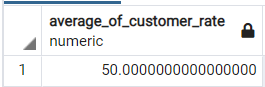
\includegraphics[width=0.5\textwidth]{figures/1.c.1.png}
    \caption
	{
پیش از آپدیت جدول \lr{rental}
	}
    \label{fig:fig1}
\end{figure}
\begin{figure}[H]
    \centering
    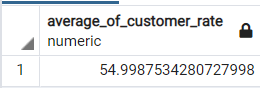
\includegraphics[width=0.5\textwidth]{figures/1.c.2.png}
    \caption
	{
پس از آپدیت جدول \lr{rental}
	}
    \label{fig:fig1}
\end{figure}


\section{2}

\section{3}
فایلِ \lr{SQL}
\section{4}

\section{5}
فایلِ \lr{SQL}
\section{6}
\begin{figure}[H]
    \centering
    
\includegraphics[width=0.5\textwidth]{figures/6.png}
    \caption
	{
سوال 6
	}
    \label{fig:fig1}
\end{figure}
\section{7}
\subsection{\lr{a}}
\subsection{\lr{b}}
\subsection{\lr{c}}
\begin{latin}
Object-Relational Mapping (ORM) is a technique that lets you query and manipulate data from a database using an object-oriented paradigm. When talking about ORM, most people are referring to a library that implements the Object-Relational Mapping technique, hence the phrase "an ORM".

An ORM library is a completely ordinary library written in your language of choice that encapsulates the code needed to manipulate the data, so you don't use SQL anymore; you interact directly with an object in the same language you're using.

\begin{itemize}
    \item [$\bullet$] Apache Cayenne, open-source for Java.
    \item [$\bullet$] Apache OpenJPA, open-source for Java.
	\item [$\bullet$] DataNucleus, open-source JDO and JPA implementation (formerly known as JPOX)
	\item [$\bullet$] Ebean, open-source ORM framework.
	\item [$\bullet$] EclipseLink, Eclipse persistence platform.
	\item [$\bullet$] Enterprise JavaBeans (EJB)
\end{itemize}
\end{latin}

\section{8}


%------------------------------------------------------------------------------------------


\section*{منابع}
\renewcommand{\section}[2]{}%
\begin{thebibliography}{99} % assumes less than 100 references
%چنانچه مرجع فارسی نیز داشته باشید باید دستور فوق را فعال کنید و مراجع فارسی خود را بعد از این دستور وارد کنید


\begin{LTRitems}

\resetlatinfont

\bibitem{b1} https://www.tutorialspoint.com/what-is-the-difference-between-blob-and-clob-datatypes
\end{LTRitems}

\end{thebibliography}


\end{document}
